\section{Цель работы}

Найти функцию, являющуюся наилучшим приближением заданной табличной функции по методу наименьших квадратов.

\section{Рабочие формулы метода}

По методу наименьших квадратов (МНК) требуется найти такую аппроксимирующую функцию $\varphi(x)$, чтобы сумма квадратов отклонений была минимальной:
\[
S = \sum_{i=1}^{n} [\varphi(x_i) - y_i]^2 \to \min
\]

\subsection{Линейная аппроксимация}

Линейная аппроксимирующая функция имеет вид $\varphi(x) = ax + b$.

Система уравнений для нахождения параметров $a$ и $b$:
\[
\begin{cases}
a \sum x_i^2 + b \sum x_i = \sum x_i y_i \\
a \sum x_i + b n = \sum y_i
\end{cases}
\]

Введём обозначения: $S_X = \sum x_i$, $S_{XX} = \sum x_i^2$, $S_Y = \sum y_i$, $S_{XY} = \sum x_i y_i$.

Решение методом Крамера:
\[
\Delta = S_{XX} \cdot n - S_X \cdot S_X,\quad
\Delta_1 = S_{XY} \cdot n - S_X \cdot S_Y,\quad
\Delta_2 = S_{XX} \cdot S_Y - S_X \cdot S_{XY}
\]
\[
a = \frac{\Delta_1}{\Delta},\quad b = \frac{\Delta_2}{\Delta}
\]

\subsection{Квадратичная аппроксимация}

Квадратичная аппроксимирующая функция имеет вид $\varphi(x) = a_0 + a_1 x + a_2 x^2$.

Система уравнений:
\[
\begin{cases}
a_0 n + a_1 \sum x_i + a_2 \sum x_i^2 = \sum y_i \\
a_0 \sum x_i + a_1 \sum x_i^2 + a_2 \sum x_i^3 = \sum x_i y_i \\
a_0 \sum x_i^2 + a_1 \sum x_i^3 + a_2 \sum x_i^4 = \sum x_i^2 y_i
\end{cases}
\]

\subsection{Среднеквадратичное отклонение}

Среднеквадратичное отклонение вычисляется по формуле:
\[
\delta = \sqrt{\frac{\sum_{i=1}^{n} (\varphi(x_i) - y_i)^2}{n}}
\]

Наилучшим считается уравнение, для которого значение $\delta$ минимально.

\section{Вычислительная часть}

Исследуемая функция (вариант 14):
\[
y = \frac{25x}{x^4 + 14},\quad x \in [0,4],\quad h = 0{,}4
\]

\subsection{Табулирование функции}

Вычислим значения функции в 11 точках интервала $[0, 4]$ с шагом $h = 0{,}4$:

\begin{table}[h!]
\centering
\label{tab:table}
\renewcommand{\arraystretch}{1.5}
\begin{tabular}{|c|c|c|c|c|c|c|c|c|c|c|c|}
\hline
$i$ & 0 & 1 & 2 & 3 & 4 & 5 & 6 & 7 & 8 & 9 & 10 \\
\hline
$x_i$ & $0{,}0$ & $0{,}4$ & $0{,}8$ & $1{,}2$ & $1{,}6$ & $2{,}0$ & $2{,}4$ & $2{,}8$ & $3{,}2$ & $3{,}6$ & $4{,}0$ \\
\hline
$y_i$ & $0{,}0000$ & $0{,}7130$ & $1{,}3880$ & $1{,}8664$ & $1{,}9461$ & $1{,}6667$ & $1{,}2718$ & $0{,}9276$ & $0{,}6731$ & $0{,}4946$ & $0{,}3704$ \\
\hline
\end{tabular}
\end{table}

\subsection{Линейная аппроксимация}

Вычислим необходимые суммы:
\[
S_X = \sum_{i=0}^{10} x_i = 0{,}0 + 0{,}4 + \cdots + 4{,}0 = 22{,}0
\]
\[
S_{XX} = \sum_{i=0}^{10} x_i^2 = 0{,}00 + 0{,}16 + \cdots + 16{,}00 = 61{,}6
\]
\[
S_Y = \sum_{i=0}^{10} y_i = 0{,}0000 + 0{,}7130 + \cdots + 0{,}3704 = 11{,}3176
\]
\[
S_{XY} = \sum_{i=0}^{10} x_i y_i = 0{,}0\cdot 0{,}0000 + 0{,}4\cdot 0{,}7130 + \cdots + 4{,}0\cdot 0{,}3704 = 21{,}1478
\]

Решаем систему уравнений:
\[
\begin{cases}
61{,}6 a + 22{,}0 b = 21{,}1478 \\
22{,}0 a + 11 b = 11{,}3176
\end{cases}
\]

Определители:
\[
\Delta = 61{,}6 \cdot 11 - 22{,}0 \cdot 22{,}0 = 677{,}6 - 484{,}0 = 193{,}6
\]
\[
\Delta_1 = 21{,}1478 \cdot 11 - 22{,}0 \cdot 11{,}3176 = 232{,}6262 - 248{,}9872 = -16{,}3610
\]
\[
\Delta_2 = 61{,}6 \cdot 11{,}3176 - 22{,}0 \cdot 21{,}1478 = 697{,}1638 - 465{,}2531 = 231{,}9107
\]

Коэффициенты:
\[
a = \frac{-16{,}3610}{193{,}6} = -0{,}0845,\quad
b = \frac{231{,}9107}{193{,}6} = 1{,}1979
\]

Линейная аппроксимирующая функция:
\[
\boxed{\varphi_{\text{лин}}(x) = -0{,}0845x + 1{,}1979}
\]

\subsection{Квадратичная аппроксимация}

Вычислим дополнительные суммы:
\[
S_{X^3} = \sum_{i=0}^{10} x_i^3 = 0{,}000 + 0{,}064 + \cdots + 64{,}000 = 193{,}6
\]
\[
S_{X^4} = \sum_{i=0}^{10} x_i^4 = 0{,}0000 + 0{,}0256 + \cdots + 256{,}0000 = 648{,}5248
\]
\[
S_{X^2Y} = \sum_{i=0}^{10} x_i^2 y_i = 49{,}1648
\]

Система уравнений:
\[
\begin{cases}
11 a_0 + 22{,}0 a_1 + 61{,}6 a_2 = 11{,}3176 \\
22{,}0 a_0 + 61{,}6 a_1 + 193{,}6 a_2 = 21{,}1478 \\
61{,}6 a_0 + 193{,}6 a_1 + 648{,}5248 a_2 = 49{,}1648
\end{cases}
\]

Решая систему методом Гаусса, получаем:
\[
a_0 = 0{,}2949,\quad a_1 = 1{,}4205,\quad a_2 = -0{,}3763
\]

Квадратичная аппроксимирующая функция:
\[
\boxed{\varphi_{\text{кв}}(x) = 0{,}2949 + 1{,}4205x - 0{,}3763x^2}
\]

\subsection{Оценка точности аппроксимаций}

Вычислим значения аппроксимирующих функций и отклонений в узлах:

\begin{table}[h!]
\centering
\label{tab:compare}
\renewcommand{\arraystretch}{1.5}
\begin{tabular}{|c|c|c|c|c|c|}
\hline
$x_i$ & $y_i$ & $\varphi_{\text{лин}}(x_i)$ & $\varepsilon_i^{\text{лин}}$ & $\varphi_{\text{кв}}(x_i)$ & $\varepsilon_i^{\text{кв}}$ \\
\hline
$0{,}0$ & $0{,}0000$ & $1{,}1979$ & $1{,}1979$ & $0{,}2949$ & $0{,}2949$ \\
$0{,}4$ & $0{,}7130$ & $1{,}1641$ & $0{,}4511$ & $0{,}8029$ & $0{,}0899$ \\
$0{,}8$ & $1{,}3880$ & $1{,}1303$ & $-0{,}2577$ & $1{,}1905$ & $-0{,}1975$ \\
$1{,}2$ & $1{,}8664$ & $1{,}0965$ & $-0{,}7699$ & $1{,}4577$ & $-0{,}4087$ \\
$1{,}6$ & $1{,}9461$ & $1{,}0627$ & $-0{,}8835$ & $1{,}6045$ & $-0{,}3417$ \\
$2{,}0$ & $1{,}6667$ & $1{,}0289$ & $-0{,}6378$ & $1{,}6309$ & $-0{,}0358$ \\
$2{,}4$ & $1{,}2718$ & $0{,}9951$ & $-0{,}2767$ & $1{,}5369$ & $0{,}2651$ \\
$2{,}8$ & $0{,}9276$ & $0{,}9613$ & $0{,}0337$ & $1{,}3225$ & $0{,}3949$ \\
$3{,}2$ & $0{,}6731$ & $0{,}9275$ & $0{,}2544$ & $0{,}9877$ & $0{,}3146$ \\
$3{,}6$ & $0{,}4946$ & $0{,}8937$ & $0{,}3990$ & $0{,}5325$ & $0{,}0378$ \\
$4{,}0$ & $0{,}3704$ & $0{,}8599$ & $0{,}4895$ & $-0{,}0431$ & $-0{,}4135$ \\
\hline
\end{tabular}
\end{table}

Вычислим среднеквадратичные отклонения:

Для линейной аппроксимации:
\[
\delta_{\text{лин}} = \sqrt{\frac{\sum_{i=0}^{10} (\varepsilon_i^{\text{лин}})^2}{11}} = \sqrt{\frac{4{,}0262}{11}} = \sqrt{0{,}3660} = 0{,}605
\]

Для квадратичной аппроксимации:
\[
\delta_{\text{кв}} = \sqrt{\frac{\sum_{i=0}^{10} (\varepsilon_i^{\text{кв}})^2}{11}} = \sqrt{\frac{0{,}9167}{11}} = \sqrt{0{,}0833} = 0{,}289
\]

\subsection{Выбор наилучшего приближения}

Сравним значения среднеквадратичных отклонений:
\[
\delta_{\text{лин}} = 0{,}605,\quad \delta_{\text{кв}} = 0{,}289
\]

Так как $\delta_{\text{кв}} < \delta_{\text{лин}}$, то \textbf{квадратичная аппроксимация является наилучшим приближением}.

\subsection{Графическая интерпретация}

На рисунке~\ref{fig:calc} представлены графики исходной функции, линейной и квадратичной аппроксимаций.

\begin{figure}[h]
    \centering
    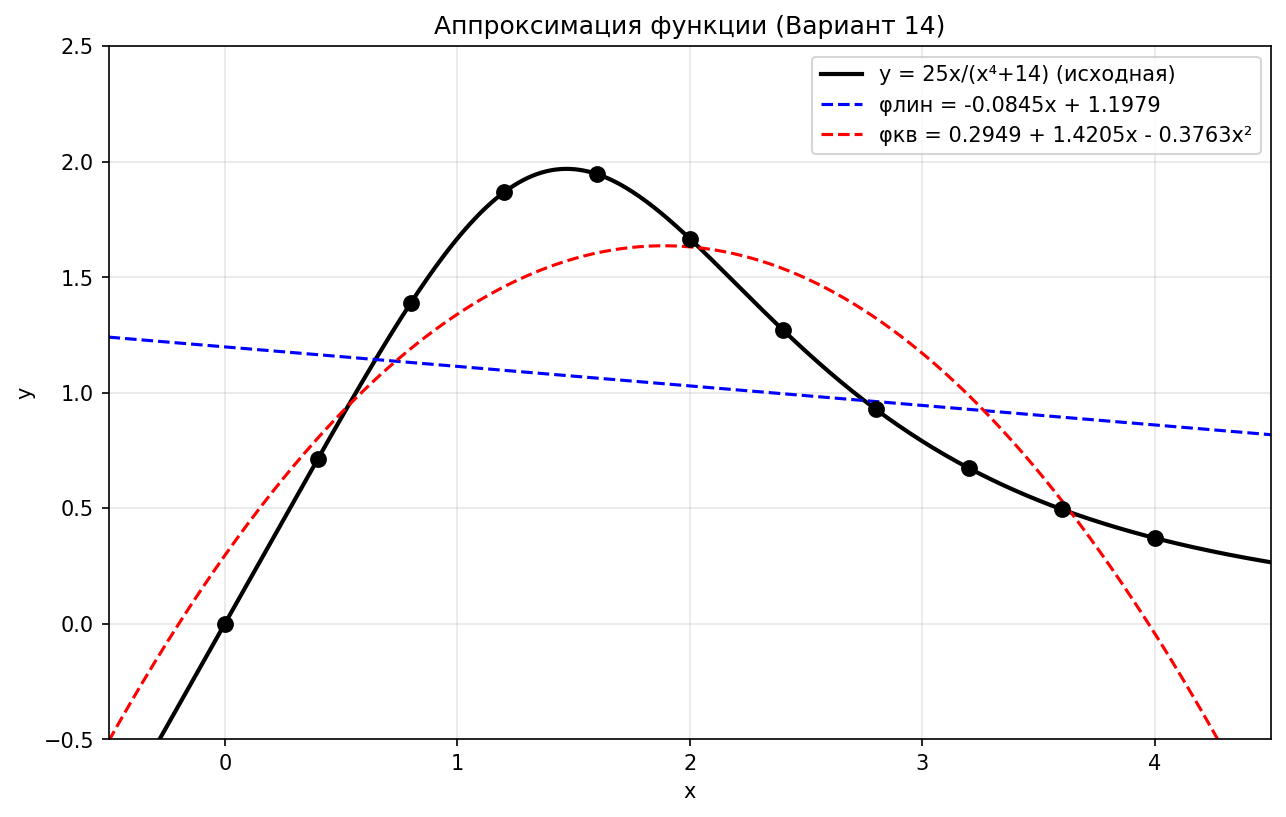
\includegraphics[width=0.9\linewidth]{pic/calc_chart.png}
    \caption{График исходной функции и аппроксимирующих функций}
    \label{fig:calc}
\end{figure}
